\chapter{Workflow}
\label{cha:workflow}
Hier wird für die behandelten \textit{major-modes} ein Workflow
vorgeschlagen. Dadurch wird eine schnelle Integration von Emacs in den
Alltag für Hardware- und Software-Entwickler möglich.\\

\section{C und C++}
\label{sec:c++}
Für den \textit{c-mode} und den \textit{c++-mode}, ist der Workflow
identisch. Es gibt zwei Punkte die beachtet werden müssen:
\begin{itemize}
\item Wird ein Projekt in der Programmiersprache C aufgesetzt, müssen
  die Endungen der Dateien von \textit{.cpp} auf \textit{.c}
  abgeändert werden.
\item In der Datei \textit{CMakelists.txt} müssen auch die Dateien
  welche eingefügt werden, von \textit{.cpp} auf \textit{.c}
  abgeändert werden.
\end{itemize}
Der Workflow für den \textit{c++-mode} ist folgendermaßen aufgebaut:
\begin{itemize}
\item Erstellen der Datei \textit{CMakelists.txt}
\item Erzeugen der Projektstruktur
\item Einfügen von Beispielcode in die Datei \textit{main.cpp}
\item Kompilieren des Projektes mit den Flaggen \textit{release} und
  \textit{debug}
\item Debuggen des Projektes
\item Löschen der generierten Dateien
\end{itemize}

\subsection{Aufsetzten und Kompilieren}
\label{subsec:projc++}
Als erstes muss zu dem Verzeichnis navigiert werden, in dem ein
Projekt erstellt werden soll. Hier wird die Datei
\textit{CMakelists.txt} angelegt. Nach dem Öffnen dieser Datei ist zu
erkennen, dass sich Emacs im \textit{cmake-mode} befindet. Nun wird
die Vorlage \textit{cmlists} mit Hilfe des Pakets \textit{yasnippet}
(siehe Abschnitt \ref{subsec:yasnippet}) aufgerufen. Dafür wird
{\glqq}cmlists{\grqq} eingetippt und am Ende die Tabulator-Taste
gedrückt. Es erscheint ein Code-Konstrukt. In dem Code-Konstrukt kann
der Name des Projektes angegeben werden und das Verzeichnis wo sich
die \textit{cpp}-Dateien befinden. Mit der Tastenkombination
\textbf{C-x C-s} wird die Datei abgespeichert. Zum Erstellen der
Ordnerstruktur wird \textbf{M-x mkdir-C-Cpp} ausgeführt. In dem
\textit{minibuffer} wird der gewünschte Name des Projektordners
eingegeben. Die Ordnerstruktur ist erstellt, folgende Ordner sind
erstellt:
\begin{itemize}
\item \textit{doc} : Für jegliche Art von Dokumenten.
\item \textit{inc} : Für alle Header-Dateien.
\item \textit{src} : Für alle Source-Dateien.
\item \textit{tests} : Für Tests.
\end{itemize}
Wurde die Ordnerstrukur erzeugt, so öffnet sich automatisch eine Datei
mit dem Namen \textit{main.cpp}. Hier kann C++-Code eingetippt
werden. Mit der Taste \textbf{<F8>} kann auf die \textit{hydra} (siehe
Abschnitt \ref{subsec:hydra}) für den \textit{c++-mode} zugegriffen
werden. Mit Hilfe der \textit{hydra} werden folgende Funktionen
ausgeführt:
\begin{itemize}
\item \textbf{<F8> b} : Ausrichten des Codes.
\item \textbf{<F8> d} : Kompilieren des Projektes mit der Flagge
  {\glqq}debug{\glqq}.
\item \textbf{<F8> r} : Kompilieren des Projektes mit der Flagge
  {\glqq}release{\glqq}.
\end{itemize}
Sind beim Kompilieren Fehler aufgetreten, müssen diese behoben werden.
Der geöffnete Puffer zeigt die Zeilen an, in denen der Fehler gefunden
wurde. Sind alle Fehler behoben, kann mit Hilfe der \textit{hydra}
(\textbf{<F8> S}), das Debugging (siehe Abschnitt
\ref{subsec:debugc++}) gestartet werden. Durch Eintippen von
    {\glqq}q{\grqq} in der Konsole wird das Debugging beendet. Nun
    werden die generierten Dateien des Projektes gelöscht. Dazu wird
    wiederum die \textit{hydra} verwendet (\textbf{<F8> C}).\\

\subsection{Debugging von C++-Code}
\label{subsec:debugc++}
Nach dem Starten des Debuggings mit der \textit{hydra} (\textbf{<F8>
  S}) öffnet sich
\textit{gdb}\footnote{\url{https://www.gnu.org/software/gdb/}} mit
sechs Fenstern. Die Abbildung \ref{fig:debug} zeigt dies an. Im
Fenster \textit{links oben} ist die \textit{gdb}-Konsole zu sehen. Mit
dieser wird das Debugging gesteuert. Darunter ist die Datei geöffnet,
in welcher sich der Debugger momentan befindet. Die aktuelle Zeile
wird mit einem Pfeil gekennzeichnet. In der Abbildung ist zu erkennen,
dass in der selben Zeile ein Haltepunkt ist. Unterhalb dieses Fensters
befindet sich eine Übersicht, in welcher Datei sich der Debugger
befindet. Auf der Abbildung ist zu sehen, dass sich der Debugger in
Zeile 40 der Datei \textit{Main.cpp} befindet. Im \textit{rechten
  oberen} Fenster werden lokale Variable angezeigt. In diesem Fenster
kann zwischen den lokalen Variablen und den Registern gewechselt
werden. Sollen komplexere Strukturen wie, Listen oder Objekte von
Klassen angezeigt werden. So werden diese in einem zusätzlichen
Fenster angezeigt. Dazu muss sich der Zeiger auf dem gewünschten
Objekt befinden und die Tastenkombination \textbf{C-c C-w} ausgeführt
werden. Es erscheint ein Rahmen mit diesem Ausdruck (zu sehen in
Abbildung \ref{fig:watch}). \textit{Unterhalb} des Fensters mit den
lokalen Ausdrücken befindet sich die Ausgabe auf der Konsole. Unter
dieser befindet sich ein Fenster mit den Haltepunkten. In diesem
Fenster kann zwischen der Anzeige der Haltepunkte und der Anzeige der
laufenden Threads gewechselt werden.\\

\begin{figure}[H]
  \centering
  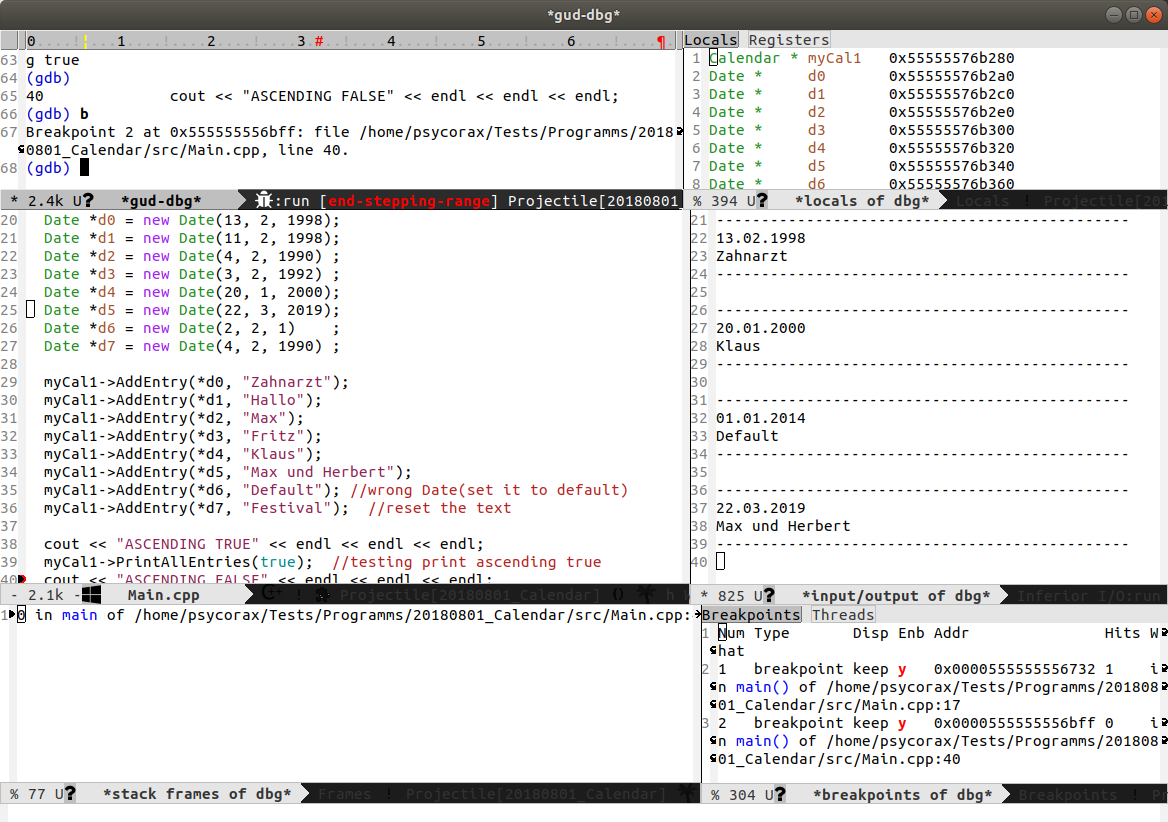
\includegraphics[width=.95\textheight, angle=90]{./images/Workflow/debugversch.png}
  \caption{\label{fig:debug} Das Debuggen in Emacs mit \textit{gdb}.}
\end{figure}

\begin{figure}[H]
  \centering
  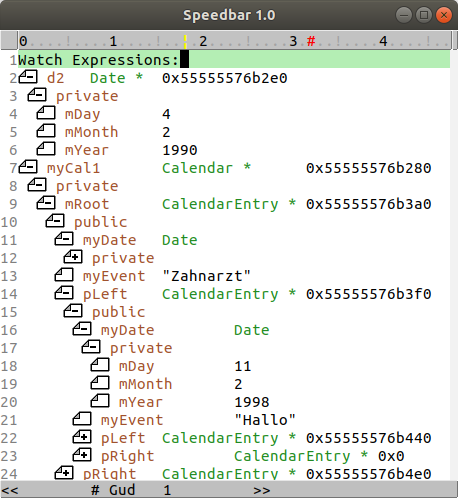
\includegraphics[width=.7\textwidth]{./images/Workflow/watch.png}
  \caption{\label{fig:watch} Diese Abbildung veranschaulicht die
    Darstellung von komplexeren Objekten in Emacs.}
\end{figure}

\section{Python}
\label{sec:python}
Der Workflow für Python ist folgendermaßen aufgebaut:
\begin{itemize}
\item Erstellen der Datei \textit{main.py}
\item Erzeugen der Projektstruktur
\item Einfügen von Beispielcode in die Datei \textit{main.py}
\item Aufruf der Python-Shell und Evaluieren des Codes
\item Wechseln zu der Python-Shell und Beenden der Python-Shell
\item Erzeugen einer ausführbaren Datei
\item Löschen der generierten Dateien
\end{itemize}

\subsection{Aufsetzten und Kompilieren des Projektes}
\label{subsec:projpython}
Als erstes wird zu dem Verzeichnis navigiert, wo das Projekt erstellt
werden soll. Hier wird die Datei \textit{main.py} angelegt. Nach dem
Öffnen dieser Datei ist zu erkennen, dass sich Emacs im
\textit{python-mode} befindet. Um die Ordnerstruktur zu erstellen wird
die Tastenkombination \textbf{M-x mkdir-py} ausgeführt. In dem
\textit{minibuffer} wird der Name des Projektes eingegeben. Nach dem
Erstellen der Ordnerstruktur kann die Datei \textit{main.py} mit Code
beschrieben werden. Für Module ist das Verzeichnis \textit{lib}
vorgesehen. Mit der Taste \textbf{<F8>} kann auf die \textit{hydra}
für den \textit{python-mode} zugegriffen werden. Mit Hilfe der
\textit{hydra} werden folgende Kombinationen ausgeführt:
\begin{itemize}
\item \textbf{<F8> b} : Ausrichten des Codes
\item \textbf{<F8> p} : Starten der Python-Shell
\item \textbf{<F8> e} : Evaluieren des Puffers in der Python-Shell
\item \textbf{<F8> s} : Die Python-Shell anzeigen\\
\end{itemize}
Die Abbildung \ref{fig:python} zeigt einen Puffer mit Python-Code und
unterhalb die Python-Shell, in der dieser Puffer ausgeführt ist. Sind
beim Evaluieren Fehler entstanden, zeigt die Python-Shell die Zeilen
an, an denen sich der Fehler befindet. Sind alle Fehler behoben, kann
mit der Option mit der \textit{hydra} eine ausführbare Datei erstellt
werden (\textbf{<F8> E}). Zum Löschen der generierten Dateien wird
ebenfalls die \textit{hydra} verwendet (\textbf{<F8> C}).\\

\begin{figure}[H]
  \centering
  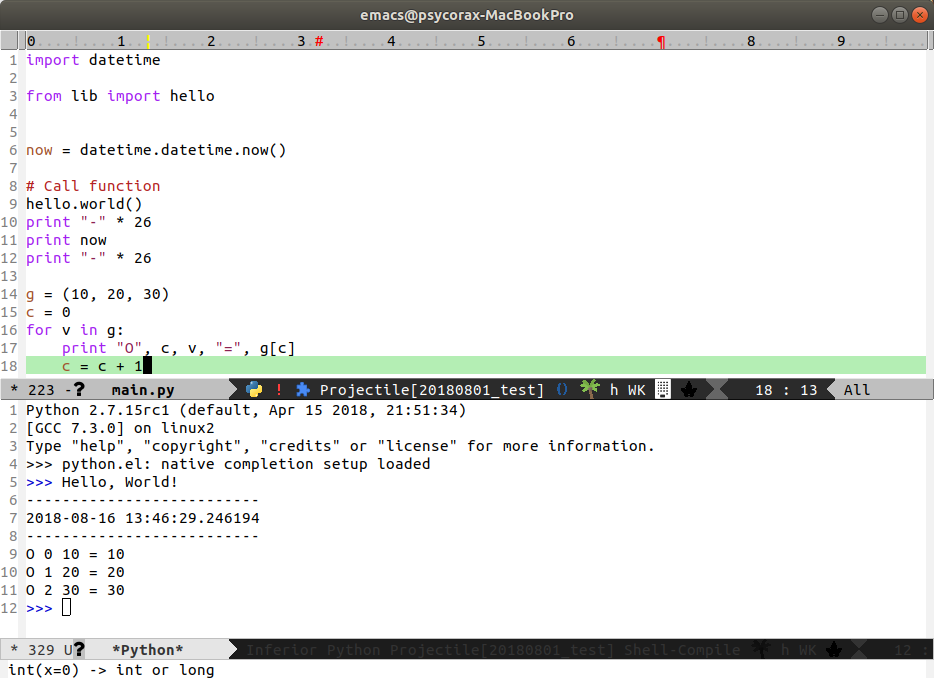
\includegraphics[width=.95\textwidth]{./images/Workflow/pythonshell.png}
  \caption{\label{fig:python} In dieser Abbildung sind ein Puffer mit
    der Datei \textit{main.py} und eine geöffnete Python-Shell zu
    sehen.}
\end{figure}

\section{Latex}
\label{sec:latex}
Der Workflow für Latex ist wie folgt aufgebaut:
\begin{itemize}
\item Erstellen einer Datei mit der Endung \textit{tex}
\item Erzeugen der Projektstruktur
\item Erzeugen der Datei \textit{Definition.tex}
\item Kompilieren des Projektes und erzeugen der \textit{PDF}-Datei
\item Löschen der generierten Dateien
\end{itemize}

\subsection{Aufsetzten und Kompilieren des Projektes}
\label{subsec:prolatex}
Als erstes wird zu dem Verzeichnis navigiert, wo das Projekt erstellt
werden soll. Hier wird eine Datei mit der Endung \textit{tex}
angelegt. Nach dem Öffnen der Datei ist zu erkennen, dass sich Emacs
im \textit{latex-mode} befindet. Nun wird die Vorlage
\textit{baseMain} mit Hilfe des Pakets \textit{yasnippet} (siehe
Abschnitt \ref{subsec:yasnippet}) aufgerufen. Dafür wird
{\glqq}baseMain{\grqq} eingetippt und am Ende der Zeichenkette die
Tabulator-Taste gedrückt. Es erscheint ein Code-Konstrukt, dieses
dient der Vorlage für eine \textit{tex}-Datei. Mit der
Tastenkombination \textbf{C-x C-s} wird die Datei abgespeichert. Zum
Erstellen der Ordnerstruktur wird die \textbf{M-x mkdir-tex}
ausgeführt. In dem \textit{minibuffer} wird der Name des Projektes
eingegeben. Für die Vorlage \textit{baseMain} wird eine zusätzliche
Datei benötigt. Diese Datei enthält die Definitionen. Die Datei
{\glqq}Definition.tex{\grqq} wird erzeugt (\textbf{C-x C-f
  Definition.tex}). Die Vorlage für diese Datei ist mit
\textit{baseDef} erreichbar. Alle benötigten Dateien zum Kompilieren
sind vorhanden. Es wird das Projekt mit der \textit{hydra} für den
\textit{latex-mode} kompiliert und eine PDF-Datei erzeugt
(\textbf{<F8> b}). Ein Fenster erscheint. In diesem sind Warnungen und
Fehler die beim Kompilieren entstanden sind aufgelistet. In der
Abbildung \ref{fig:latex} ist im oberen Fenster der Puffer mit der
\textit{Latex}-Datei zu sehen und unterhalb das Fenster mit den
Warnungen und Fehlern. Sind keine Fehler vorhanden, so wird die
PDF-Datei generiert. Die Tastenkombination \textbf{<F8> C} löscht den
Ordner \textit{build} und damit alle generierten Dateien.\\

\begin{figure}[h]
  \centering
  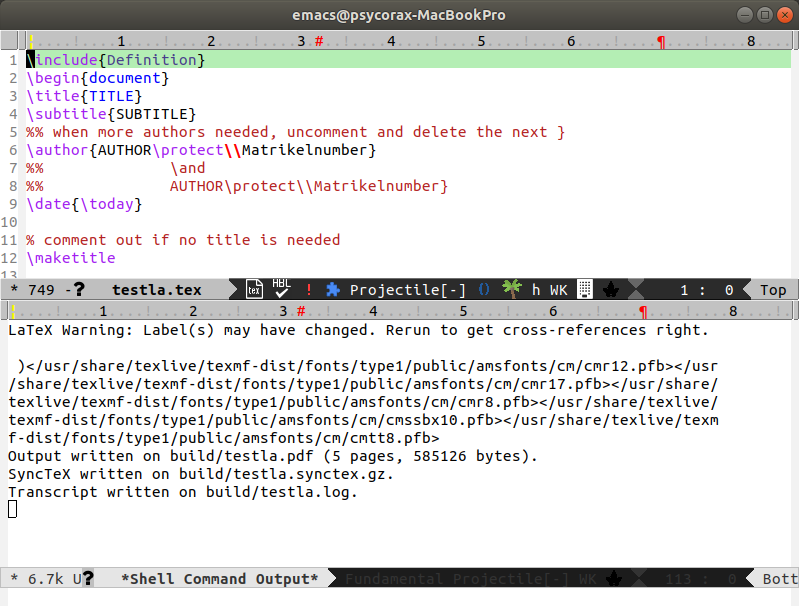
\includegraphics[width=.95\textwidth]{./images/Workflow/latex.png}
  \caption{\label{fig:latex} Kompilieren des \textit{latex}-Projektes.}
\end{figure}

\section{VHDL}
\label{sec:vhdl}
Für den Modus \textit{vhdl-mode} ist der Workflow wie folgt aufgebaut:
\begin{itemize}
\item Erstellen einer Datei mit der Endung \textit{vhd}
\item Erzeugen der Projektstruktur
\item Einfügen von Beispielcode in die \textit{vhd}-Datei
\item Den Code mit
  \textit{ghdl}\footnote{\url{https://github.com/ghdl/ghdl}}
  kompilieren
\item Erzeugen einer \textit{tcl}-Datei
\item Diese \textit{tcl}-Datei zum Start für
  \textit{Modelsim}\footnote{\url{https://www.intel.com/content/www/us/en/software/programmable/quartus-prime/model-sim.html}}
  definieren
\item Starten von \textit{Modelsim} und Ausführen des
  \textit{tcl}-Skriptes
\item Löschen der generierten Dateien
\end{itemize}

\subsection{Aufsetzten und Kompilieren des Projektes}
Als erstes wird zu dem Verzeichnis navigiert, wo das Projekt erstellt
werden soll. Hier wird eine Datei mit der Endung \textit{vhd}
erstellt. Nach dem Öffnen dieser Datei ist zu erkennen, dass sich
Emacs im Modus \textit{vhdl-mode} befindet. Die Projektstruktur wird
erstellt (\textbf{M-x mkdir-vhdl}). In dem Ordner \textit{sim} werden
\textit{tcl}-Datein für das Projekt gesammelt. Eine solche Datei wird
angelegt (\textbf{C-x C-f mysim.tcl}). In der \textit{mode-line} ist
zu erkennen, dass sich Emacs im \textit{tcl-mode} befindet. Nun wird
die Vorlage \textit{tcl} mit Hilfe des Pakets \textit{yasnippet}
(siehe Abschnitt \ref{subsec:yasnippet}) eingefügt. Dafür wird
{\glqq}tcl{\grqq} eingetippt und am Ende der Zeichenkette die
Tabulator-Taste gedrückt. Es erscheint ein Code-Konstrukt, welches als
Vorlage für \textit{tcl}-Dateien zum Kompilieren und Simmulieren
mittels \textit{modelsim} dient. Nachdem alle Dateinamen korrekt
eingefügt sind, wird die Datei abgespeichert (\textbf{C-x C-s}). Der
\textit{src}-Ordner ist für die \textit{vhd}-Dateien vorgesehen. Mit
der \textit{hydra} für den \textit{vhdl-mode} werden folgende
Funktionen ausgeführt:
\begin{itemize}
\item \textbf{<F8> b} : Ausrichten des Codes
\item \textbf{<F8> c} : Kompilieren mit Hilfe von \textit{ghdl}
\item \textbf{<F8> s} : Festlegen der verwendeten\textit{tcl}-Datei
  für \textit{Modelsim}
\item \textbf{<F8> S} : Starten von \textit{Modelsim} und Ausführen
  des \textit{tcl}-Skriptes\\
\end{itemize}
Beim Kompilieren mit \textit{ghdl} kann die Syntax für den momentan
angezeigten Puffer überprüft werden (in Abbildung \ref{fig:ghdl} zu
sehen). Die Simulation mit \textit{Modelsim} basiert auf dem
definierten \textit{tcl}-Skript. Zum Löschen der generierten Dateien
wird die \textit{hydra} verwendet (\textit{<F8> C}).\\

\begin{figure}[h]
  \centering
  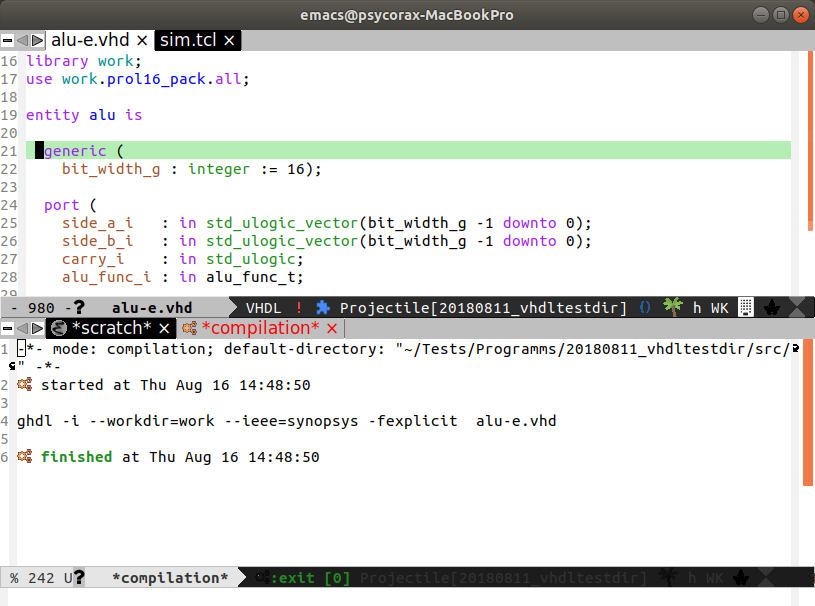
\includegraphics[width=.95\textwidth]{./images/Workflow/ghdl.png}
  \caption{\label{fig:ghdl} Kompilieren des Puffers mit \textit{ghdl}.}
\end{figure}
